\documentclass[11pt,a4paper]{article}

\usepackage[margin=2.5cm]{geometry}
\usepackage[utf8]{inputenc}
\usepackage[spanish]{babel}
\usepackage{graphicx}
\usepackage{amsmath}
\usepackage{hyperref}
\usepackage{booktabs}
\usepackage{enumitem}
\usepackage{titlesec}
\usepackage{caption}
\usepackage{subcaption}
\usepackage{float}

\titleformat{\section}{\large\bfseries}{\thesection}{1em}{}
\titleformat{\subsection}{\normalsize\bfseries}{\thesubsection}{1em}{}

\title{Métodos Basados en el Conocimiento Aplicado a Empresas (CAE)\\
       Módulo de Cuantificación}

\author{
Estudiante: Juan Camilo España Lopera\\
Profesor: Jose Ramón Quevedo Pérez\\[6pt]
Universidad de Oviedo
}

\date{\today}

% ─────────────────────────────────────────────────────────────────────────────
\begin{document}
\maketitle


% =============================================================================
\section{Contexto y motivación}
% =============================================================================

Una empresa de consultoría de IA necesita saber qué tan seguido un modelo de
lenguaje (LLM) produce información incorrecta (\textit{alucinaciones}) cuando
genera recomendaciones médicas. Contratar expertos que revisen cada
recomendación una a una es muy costoso, por lo que se busca un método
que estime directamente el \textbf{porcentaje de alucinaciones} en un lote de
recomendaciones sin necesidad de revisarlas todas.

Cada recomendación está etiquetada individualmente con una variable binaria
$y_{\text{al},i} \in \{0, 1\}$: vale $1$ si la recomendación contiene una
alucinación y $0$ si es válida. Lo que se quiere estimar no es el valor de
$y_{\text{al},i}$ para cada recomendación, sino la \textbf{prevalencia} del
conjunto: la fracción de recomendaciones con $y_{\text{al},i} = 1$ dentro
de un lote.

Para ello se dispone de tres conjuntos de datos, donde cada recomendación
está descrita por 10 características de texto calculadas automáticamente
(número de palabras, diversidad léxica, densidad de cifras, etc.):

\begin{table}[H]
\centering
\caption{Conjuntos de datos disponibles}
\begin{tabular}{lccl}
\toprule
\textbf{Dataset} & \textbf{Muestras} & \textbf{Prevalencia real} & \textbf{Rol} \\
\midrule
E1 & 418 & 0.15 (15\,\%) & Entrenamiento \\
E2 & 255 & 0.25 (25\,\%) & Evaluación (LLM diferente) \\
E3 & 313 & Desconocida   & Producción \\
\bottomrule
\end{tabular}
\end{table}

E2 proviene de una versión diferente del LLM, por lo que tiene una prevalencia
y un patrón de alucinaciones distinto. En consecuencia, un método entrenado
en E1 no funcionará bien en E2 si asume la misma distribución. Esta situación
se repetirá con conjuntos futuros, ya que los LLMs propietarios se actualizan
continuamente y modifican sus patrones de alucinación.


% =============================================================================
\section{Definición del problema}
% =============================================================================

El objetivo es estimar la prevalencia $\hat{p}$ en un lote de $n$
recomendaciones, es decir, qué fracción de ellas contiene alucinaciones:

\begin{equation}
    \hat{p} = \frac{1}{n}\sum_{i=1}^{n} y_{\text{al},i}
\end{equation}

donde $y_{\text{al},i} \in \{0,1\}$ es la etiqueta binaria de la
recomendación $i$. En lugar de predecir $y_{\text{al},i}$ para cada
recomendación, se estima directamente $\hat{p}$ del lote. Esto es útil
cuando lo que importa es la proporción, no los casos individuales.

La dificultad principal es que E2 tiene mayor prevalencia que E1
(25\,\% vs.\ 15\,\%): los métodos entrenados en E1 no pueden asumir que
la distribución se mantiene igual en E2 ni en E3.


% =============================================================================
\section{Preprocesamiento}
% =============================================================================

Cada conjunto de datos contiene 10 atributos numéricos por recomendación:
\texttt{n\_words}, \texttt{n\_refs}, \texttt{lex\_div}, \texttt{hedge\_r},
\texttt{spec\_sc}, \texttt{sent\_pol}, \texttt{consist}, \texttt{src\_dens},
\texttt{num\_dens}, \texttt{verb\_ten}.

Se comprobó la ausencia de valores nulos y que los atributos están en escalas
similares. Dado que el clasificador base (Random Forest) no depende de la
escala, no se aplica normalización adicional.


% =============================================================================
\section{Métodos de cuantificación}
% =============================================================================

Se prueban cuatro métodos, todos entrenados con E1 y evaluados en E2:

\subsection*{CC — Classify and Count}
Clasifica cada recomendación y cuenta cuántas predice como alucinación.
Es el método más sencillo, pero subestima o sobreestima la prevalencia
cuando el conjunto de evaluación tiene una distribución diferente al de
entrenamiento.

\subsection*{AC — Adjusted Count}
Igual que CC, pero corrige el conteo usando las tasas de error del
clasificador (falsos positivos y falsos negativos). Reduce el sesgo cuando
la prevalencia cambia, pero la corrección sigue dependiendo del clasificador.

\subsection*{PAC — Probabilistic Adjusted Count}
Variante de AC que usa las probabilidades del clasificador en lugar de sus
predicciones directas. Suele ser más estable que AC cuando el clasificador
está bien calibrado.

\subsection*{DFX — Distribution y-similarity}
No usa el clasificador directamente. Compara la distribución del lote con
distribuciones de referencia de cada clase, y elige la prevalencia que hace
que la mezcla se parezca más al lote observado. Tiene dos parámetros:
número de intervalos del histograma (\texttt{n\_bins}) y función de
distancia (\texttt{L1}, \texttt{L2} o \texttt{HD}).


% =============================================================================
\section{Selección de modelos}
% =============================================================================

\subsection{Clasificador base (Random Forest)}

Se entrena un Random Forest de 100 árboles sobre E1. En E1 el clasificador
casi no comete errores (sobreajuste esperado); lo relevante es su
comportamiento en E2.

\begin{figure}[H]
    \centering
    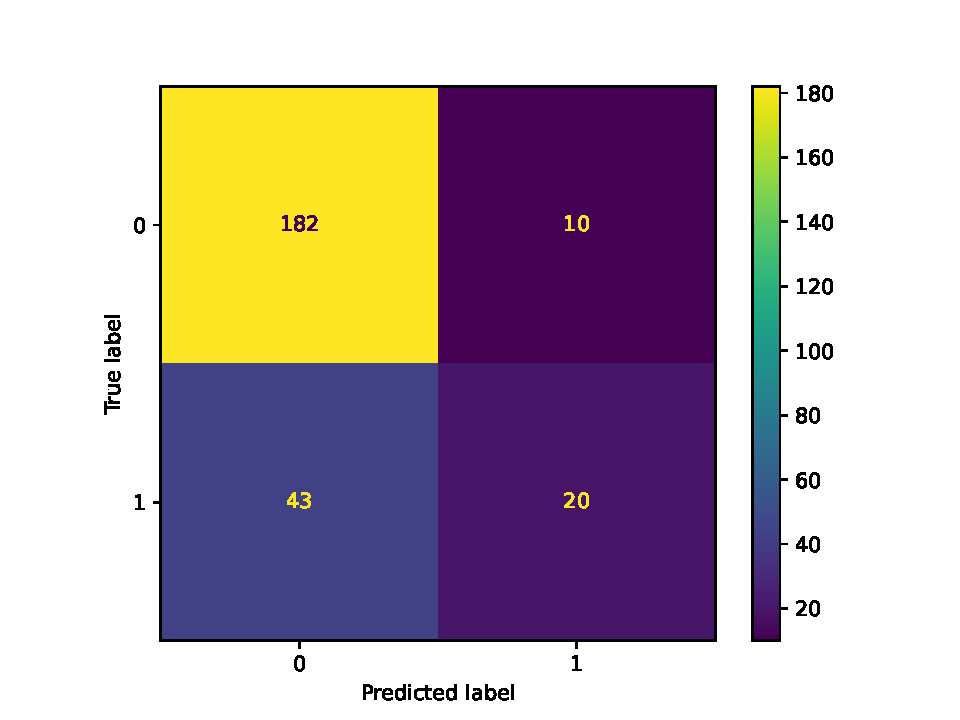
\includegraphics[width=0.55\textwidth]{figures/confusion_E2.pdf}
    \caption{Matriz de confusión del Random Forest evaluado sobre E2.
             Las filas indican la clase real ($y_{\text{al},i}$) y las
             columnas la predicción. Los errores fuera de la diagonal
             muestran los fallos del clasificador en E2.}
    \label{fig:confusion}
\end{figure}

El clasificador comete más errores en E2 que en E1 porque fue entrenado con
una prevalencia del 15\,\% y en E2 la prevalencia real es del 25\,\%.
Esta limitación motiva el uso de cuantificadores que corrijan ese sesgo.


% =============================================================================
\section{Metodología experimental}
% =============================================================================

El proceso experimental tuvo tres pasos:

\begin{enumerate}
    \item \textbf{Comparación directa en E2:} Cada método estima $\hat{p}$
    usando E2 completo (255 muestras). Se compara con la prevalencia real
    (0.25) usando el error absoluto ($L_1$) y el error cuadrático ($L_2$).
    Cuanto más cerca de cero, mejor.

    \item \textbf{Afinamiento del mejor método:} DFX obtuvo el menor error
    en el paso anterior, por lo que se busca su mejor configuración de
    parámetros con Optuna (200 combinaciones). Solo se afina el mejor
    candidato para reducir el costo computacional.

    \item \textbf{Prueba de robustez con bags:} Se generan 200 submuestras
    de E2 con prevalencias variadas entre 0 y 1. Se mide el error $L_1$ de
    DFX afinado en cada submuestra para comprobar si funciona bien ante
    distintos niveles de prevalencia.
\end{enumerate}


% =============================================================================
\section{Evaluación de resultados}
% =============================================================================

\subsection{Comparación directa de los cuatro métodos en E2}

La siguiente tabla muestra la estimación de $\hat{p}$ de cada método sobre
E2 (prevalencia real: 0.25) y su error:

\begin{table}[H]
\centering
\caption{Estimaciones de prevalencia en E2 y errores (valor real: 0.25)}
\begin{tabular}{lccc}
\toprule
\textbf{Método} & $\hat{p}$ & Error $L_1$ & Error $L_2$ \\
\midrule
CC         & 0.1176 & 0.1294 & 0.0167 \\
AC         & 0.1176 & 0.1294 & 0.0167 \\
PAC        & 0.1975 & 0.0496 & 0.0025 \\
DFX (base) & 0.2201 & 0.0269 & 0.0007 \\
\bottomrule
\end{tabular}
\end{table}

CC y AC producen la misma estimación (0.12), subestimando la prevalencia real.
PAC mejora al usar probabilidades del clasificador, y DFX obtiene el error
más bajo al no depender del sesgo del clasificador. La
figura~\ref{fig:scatter} muestra esta diferencia visualmente.

\begin{figure}[H]
    \centering
    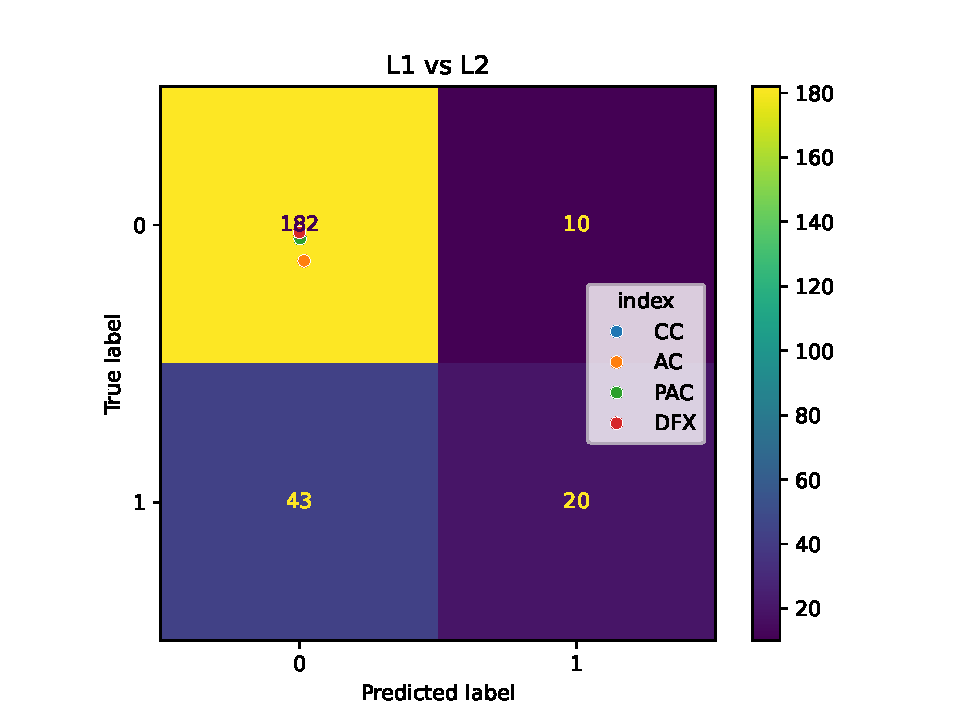
\includegraphics[width=0.6\textwidth]{figures/scatter_L1_L2.pdf}
    \caption{Error $L_1$ vs.\ $L_2$ de cada método en E2. CC y AC se
             superponen en la esquina superior derecha (mayor error). PAC
             mejora ambos errores y DFX queda más cerca del origen,
             confirmando que es el método más preciso.}
    \label{fig:scatter}
\end{figure}


\subsection{Afinamiento de hiperparámetros de DFX}

Se busca la mejor combinación de \texttt{n\_bins} $\in [10, 200]$ y
\texttt{distance} $\in \{\text{L1, L2, HD}\}$ con Optuna (200 intentos),
minimizando el error $L_1$ sobre E2.

La mejor configuración fue $\texttt{n\_bins} = 28$ y
$\texttt{distance} = \text{L1}$, con un error $L_1 = 0.0015$ — frente a
$L_1 = 0.0269$ del DFX sin afinar.

\begin{figure}[H]
    \centering
    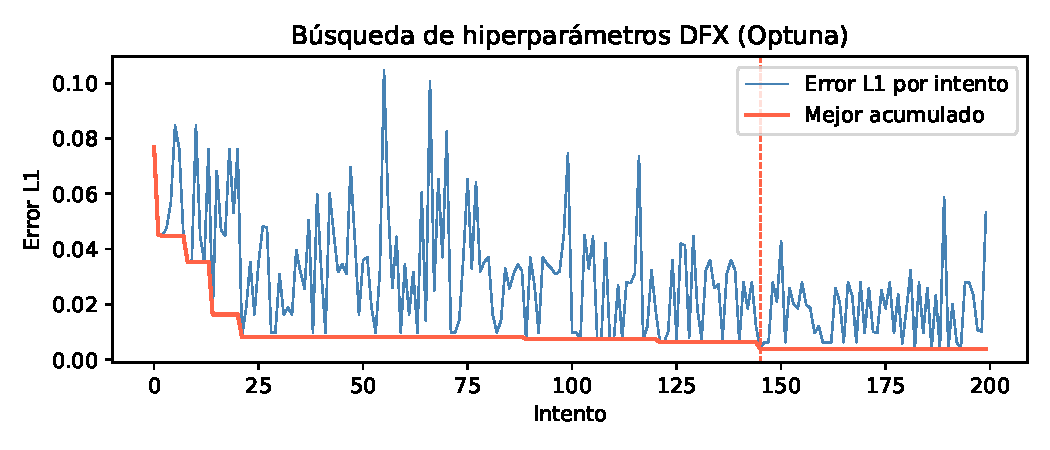
\includegraphics[width=0.72\textwidth]{figures/optuna_history.pdf}
    \caption{Evolución del error $L_1$ en los 200 intentos de Optuna.
             La línea azul muestra el error de cada intento y la roja el
             mejor valor acumulado. La línea discontinua marca el intento
             con la mejor configuración encontrada.}
    \label{fig:optuna}
\end{figure}

La curva roja cae rápidamente en los primeros intentos y se estabiliza,
lo que indica que 200 intentos son suficientes para encontrar una buena
configuración.


\subsection{Robustez de DFX afinado (bags)}

Para evaluar si DFX funciona bien en distintos niveles de prevalencia,
no solo en el valor puntual de E2, se generan 200 submuestras con
prevalencias variadas entre 0 y 1 sobre E2.

\begin{table}[H]
\centering
\caption{Error $L_1$ de DFX afinado en los 200 bags de E2}
\begin{tabular}{cccc}
\toprule
$L_1$ medio & Desv.\ típica & $L_1$ mínimo & $L_1$ máximo \\
\midrule
0.1147 & 0.0839 & 0.0007 & 0.3357 \\
\bottomrule
\end{tabular}
\end{table}

El error medio (0.11) es mayor que sobre E2 completo (0.0015) porque los
bags incluyen prevalencias extremas (cercanas a 0 o a 1) que son más
difíciles de estimar con pocos datos. En el rango central el modelo funciona
bien, como muestra la figura~\ref{fig:bags}.

\begin{figure}[H]
    \centering
    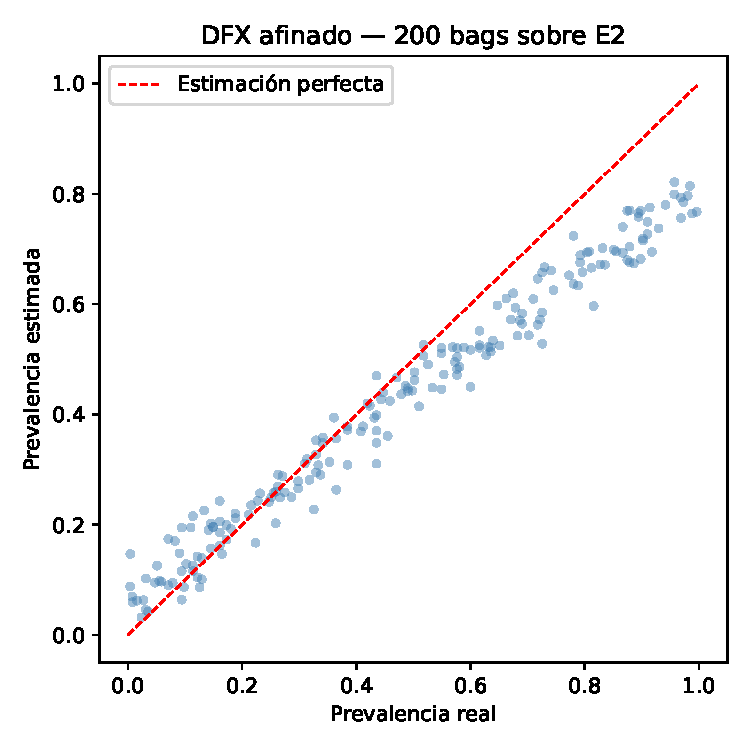
\includegraphics[width=0.52\textwidth]{figures/bags_scatter.pdf}
    \caption{Prevalencia real vs.\ estimada por DFX afinado en los 200 bags
             de E2. La línea roja discontinua representa la estimación
             perfecta. La mayor dispersión en los extremos refleja la
             dificultad de estimar prevalencias muy altas o muy bajas.}
    \label{fig:bags}
\end{figure}


% =============================================================================
\section{Paso a producción}
% =============================================================================

Una vez seleccionado DFX afinado ($\texttt{n\_bins}=28$,
$\texttt{distance}=\text{L1}$) como mejor método, se reentrena combinando
E1 y E2 (673 muestras en total) para aprovechar todos los datos etiquetados
disponibles. Este modelo final se aplica sobre E3.

La prevalencia estimada en E3 es:

\begin{equation}
    \hat{p}_{E3} = 0.2986 \quad (29.9\,\%)
\end{equation}

El modelo estima que aproximadamente \textbf{3 de cada 10 recomendaciones}
del tercer LLM contienen una alucinación. La prevalencia real de E3 es 0.35
(35\,\%), lo que da un error $L_1 = 0.05$, del mismo orden que el obtenido
sobre E2, confirmando que el método generaliza de forma consistente a nuevas
versiones del LLM.


% =============================================================================
\section{Conclusiones}
% =============================================================================

\begin{itemize}
    \item \textbf{CC y AC fallan ante el cambio de prevalencia:} Ambos
    estimaron $\hat{p} = 0.12$ en E2 (real: 0.25), con un error
    $L_1 = 0.13$. CC no corrige el sesgo del clasificador, y AC no logra
    compensarlo porque su corrección fue calculada sobre E1.

    \item \textbf{PAC reduce el error a la mitad:} Al usar probabilidades
    en lugar de predicciones directas, PAC estimó $\hat{p} = 0.20$
    ($L_1 = 0.05$) sin cambiar el clasificador base.

    \item \textbf{DFX es el método más preciso:} Al comparar distribuciones
    en lugar de contar predicciones, DFX base obtuvo $L_1 = 0.027$. Tras
    el afinamiento con Optuna ($\texttt{n\_bins}=28$,
    $\texttt{distance}=\text{L1}$) el error bajó a $L_1 = 0.0015$ en E2.

    \item \textbf{Generalización a E3:} El modelo final estimó
    $\hat{p}_{E3} = 0.30$ frente al valor real de 0.35 ($L_1 = 0.05$),
    confirmando que DFX afinado funciona bien en nuevas versiones del LLM
    sin necesidad de reetiquetar datos.
\end{itemize}

\end{document}
